\documentclass[11pt]{article}

\usepackage{fullpage}
\usepackage{graphicx}
\usepackage{amsmath}
\usepackage{amssymb}
\usepackage{amsthm}
\usepackage{fancyvrb}

\parindent0in
\pagestyle{plain}
\thispagestyle{plain}

\newcommand{\myname}{Mehshan Mustafa}
\newcommand{\dated}{\today}

\newenvironment{theorem}[2][Theorem]{\begin{trivlist}
\item[\hskip \labelsep {\bfseries #1}\hskip \labelsep {\bfseries #2.}]}{\end{trivlist}}
\newenvironment{lemma}[2][Lemma]{\begin{trivlist}
\item[\hskip \labelsep {\bfseries #1}\hskip \labelsep {\bfseries #2.}]}{\end{trivlist}}
\newenvironment{exercise}[2][Exercise]{\begin{trivlist}
\item[\hskip \labelsep {\bfseries #1}\hskip \labelsep {\bfseries #2.}]}{\end{trivlist}}
\newenvironment{problem}[2][Problem]{\begin{trivlist}
\item[\hskip \labelsep {\bfseries #1}\hskip \labelsep {\bfseries #2.}]}{\end{trivlist}}
\newenvironment{question}[2][Question]{\begin{trivlist}
\item[\hskip \labelsep {\bfseries #1}\hskip \labelsep {\bfseries #2.}]}{\end{trivlist}}
\newenvironment{corollary}[2][Corollary]{\begin{trivlist}
\item[\hskip \labelsep {\bfseries #1}\hskip \labelsep {\bfseries #2.}]}{\end{trivlist}}
\newenvironment{solution}{\begin{proof}[Solution]}{\end{proof}}
\newenvironment{idea}[2][Proof Idea.]{\textit{#1} #2}

\begin{document}

\textbf{Introduction to the Theory of
Computation}\hfill\textbf{\myname}\\[0.01in]
\textbf{Chapter 1: Reqular Languages}\hfill\textbf{\dated}\\
\smallskip\hrule\bigskip

\begin{problem}{1.67}
Let the rotational closure of language $A$ be $RC(A) = \{yx \; | \; xy \in A\}$.
\end{problem}

\begin{problem}[Part]{a}
Show that for any language $A$, we have $RC(A) = RC(RC(A))$.
\end{problem}

\begin{proof}
abc

abc     y's = a[bc], ab[c], abc[]
bca	y's = b[ca], bc[a], bca[]
cab	y's = c[ab], ca[b], cab[]


there are n possible values for y... n1, n1.n2, ..... n1.n2.....nn    n is length of a string in the language....

w=w1w2....wn

because there are n possible values for y... therefore there are n rotations for each w, n = |w|......

w2w3.....wnw1
..
..
..
wnw1w2....w(n-1)
w=w1w2....wn

these rotations ar cyclical.. have same length as the original string w .... and have the same.. applying the rotation operation on any of the rotated string does not generate any new string.

any rotated string is rotate n times...  show that:
R(w) = R(wr) ... where wr is in R(w)

\end{proof}

\begin{problem}[Part]{b}
Show that the class of regular languages is closed under rotational closure.
\end{problem}

\begin{idea}

\begin{center}
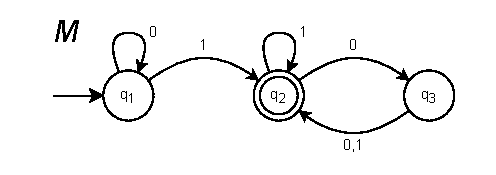
\includegraphics[scale=1.0]{Figures/Problem1.67a.pdf} \\
State diagram of DFA $M$ that recognizes A. $A = \{w \ | \ w \ contains \ at \ least \ one \ 1 \ and \ an \ even \ number \ of \ 0s \ follow \ the \ last \ 1\}$.
\end{center}

\begin{center}
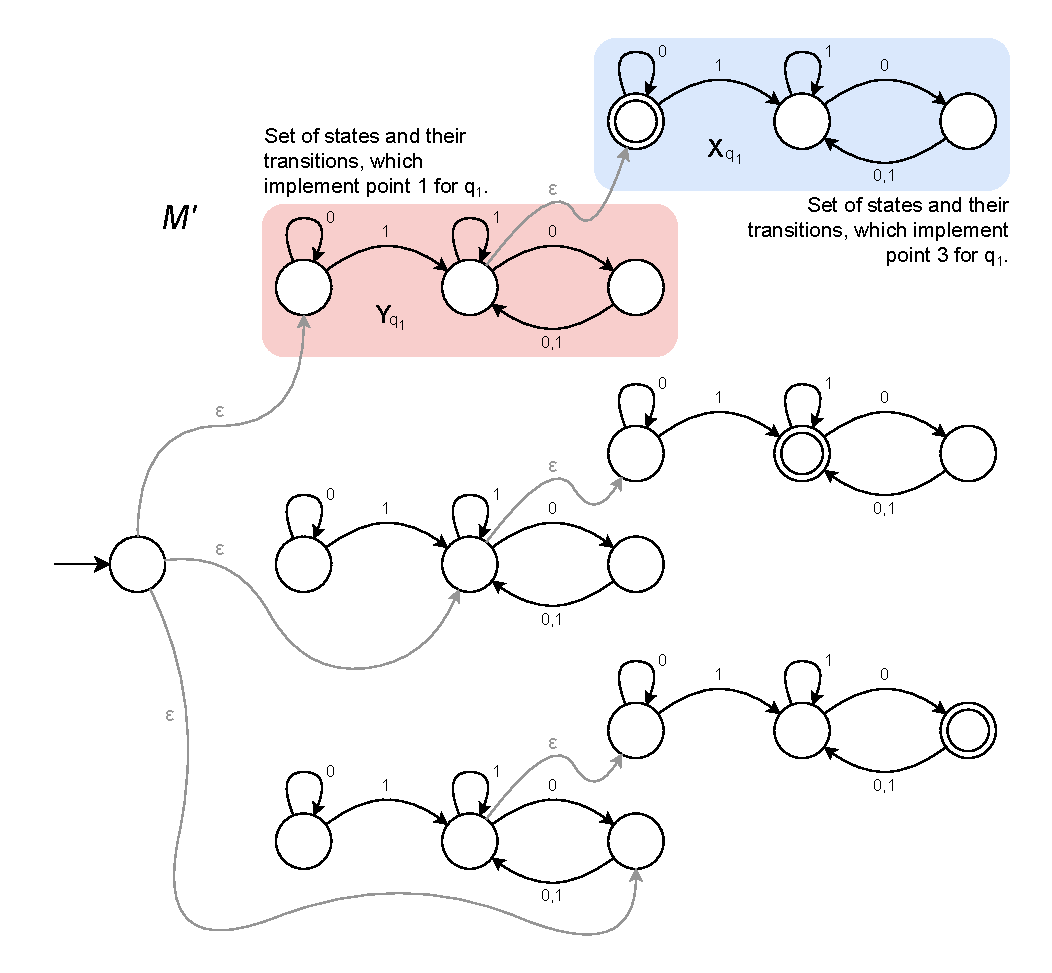
\includegraphics[scale=0.75]{Figures/Problem1.67b.pdf} \\
State diagram of DFA $M'$ that recognizes $RC(A)$.
\end{center}

\end{idea} 

\begin{proof}
Let $M = (Q, \Sigma, \delta, q_{0}, F)$ be the DFA that recognizes $A$. Construct the NFA $M' = (Q', \Sigma, \delta', q_{0}', F')$ to recognize $RC(A)$.
\begin{enumerate}
\item $Q' = Q_{s} \cup Q_{x} \cup Q_{y}$, where
\[ 
Q_{s} = \{ q_{s} \} \ , \ Q_{x} = \bigcup_{i=1}^{|Q|}X_{q_{i}} \ , \ Q_{y} = \bigcup_{i=1}^{|Q|}Y_{q_{i}}
\]
For each $q \in Q$
\[
X_{q_{i}} = \{(q_{i}, x, q_{1}), (q_{i}, x, q_{2}), \cdots , (q_{i}, x, q_{n})\}
\]
\[
Y_{q_{i}} = \{(q_{i}, y, q_{1}), (q_{i}, y, q_{2}), \cdots , (q_{i}, y, q_{n})\}
\]
The state $q_{s}$ is the new start state. For every state in the DFA $M$, there are two copies of M....
\item $q_{0}' = q_{s}$
\item $F' = \{ (q_{1}, x, q_{1}), (q_{2}, x, q_{2}), \cdots, (q_{n}, x, q_{n})  \}$, where each $q_{i} \in Q$.
\item Define $\delta'$(q, a) so that for any $q \in Q'$ and any $a \in \Sigma_{\epsilon}$: $q = (q_{i},x,q_{j})$
\begin{center}
$\displaystyle \delta '( q,\ a) \ =\begin{cases}
\{(q_{1}, y, q_{1}), (q_{2}, y, q_{2}),\cdots,(q_{n}, y, q_{n})\} & q=q_{s} \ and\ a\ =\ \epsilon \\
\{(q_{i},x,\delta(q_{j},a))\}  & q \in Q_{x} \\
\{(q_{i},y,\delta(q_{j},a))\}  & q \in Q_{y} \ and \ q_{j} \notin F \\
\{(q_{i},y,\delta(q_{j},a))\}  & q \in Q_{y}, \ q_{j} \in F \ and \ a \neq \epsilon \\
\{(q_{i},x,q_{0})\}  & q \in Q_{y}, \ q_{j} \in F \ and \ a = \epsilon \\
\end{cases} \ \ $
\end{center}
\end{enumerate}
\end{proof}

\end{document}